\chapter{Sef}

Sef predstavlja posljednju komponentu sustava za kontrolu pristupa.
Sastoji se od nekolicine elektroničkih komponenti i upravljačkog softvera (eng. \textit{firmware}).

U ovom poglavlju komponente i softver će biti opisani i razrađeni.

\section{Komponente}

Sef zahtjeva različite komponente kako bi ispunio svoju zadaću.
Komponente su povezane s mikrokontrolerom koji upravlja s istima.
U nastavku je popis potrebnih komponenti s kratkim opisom.

\subsection{ESP32}

Koristi se izvedba ESP32 pločice tvrtke \textit{WEMOS}, model \textit{D32}.
Sadrži 22 digitalna i 8 analognih pinova, a radi na 3.3V\@.
Procesorska jedinica radi na brzini do 240MHz.

\begin{figure}[h!]
    \centering
    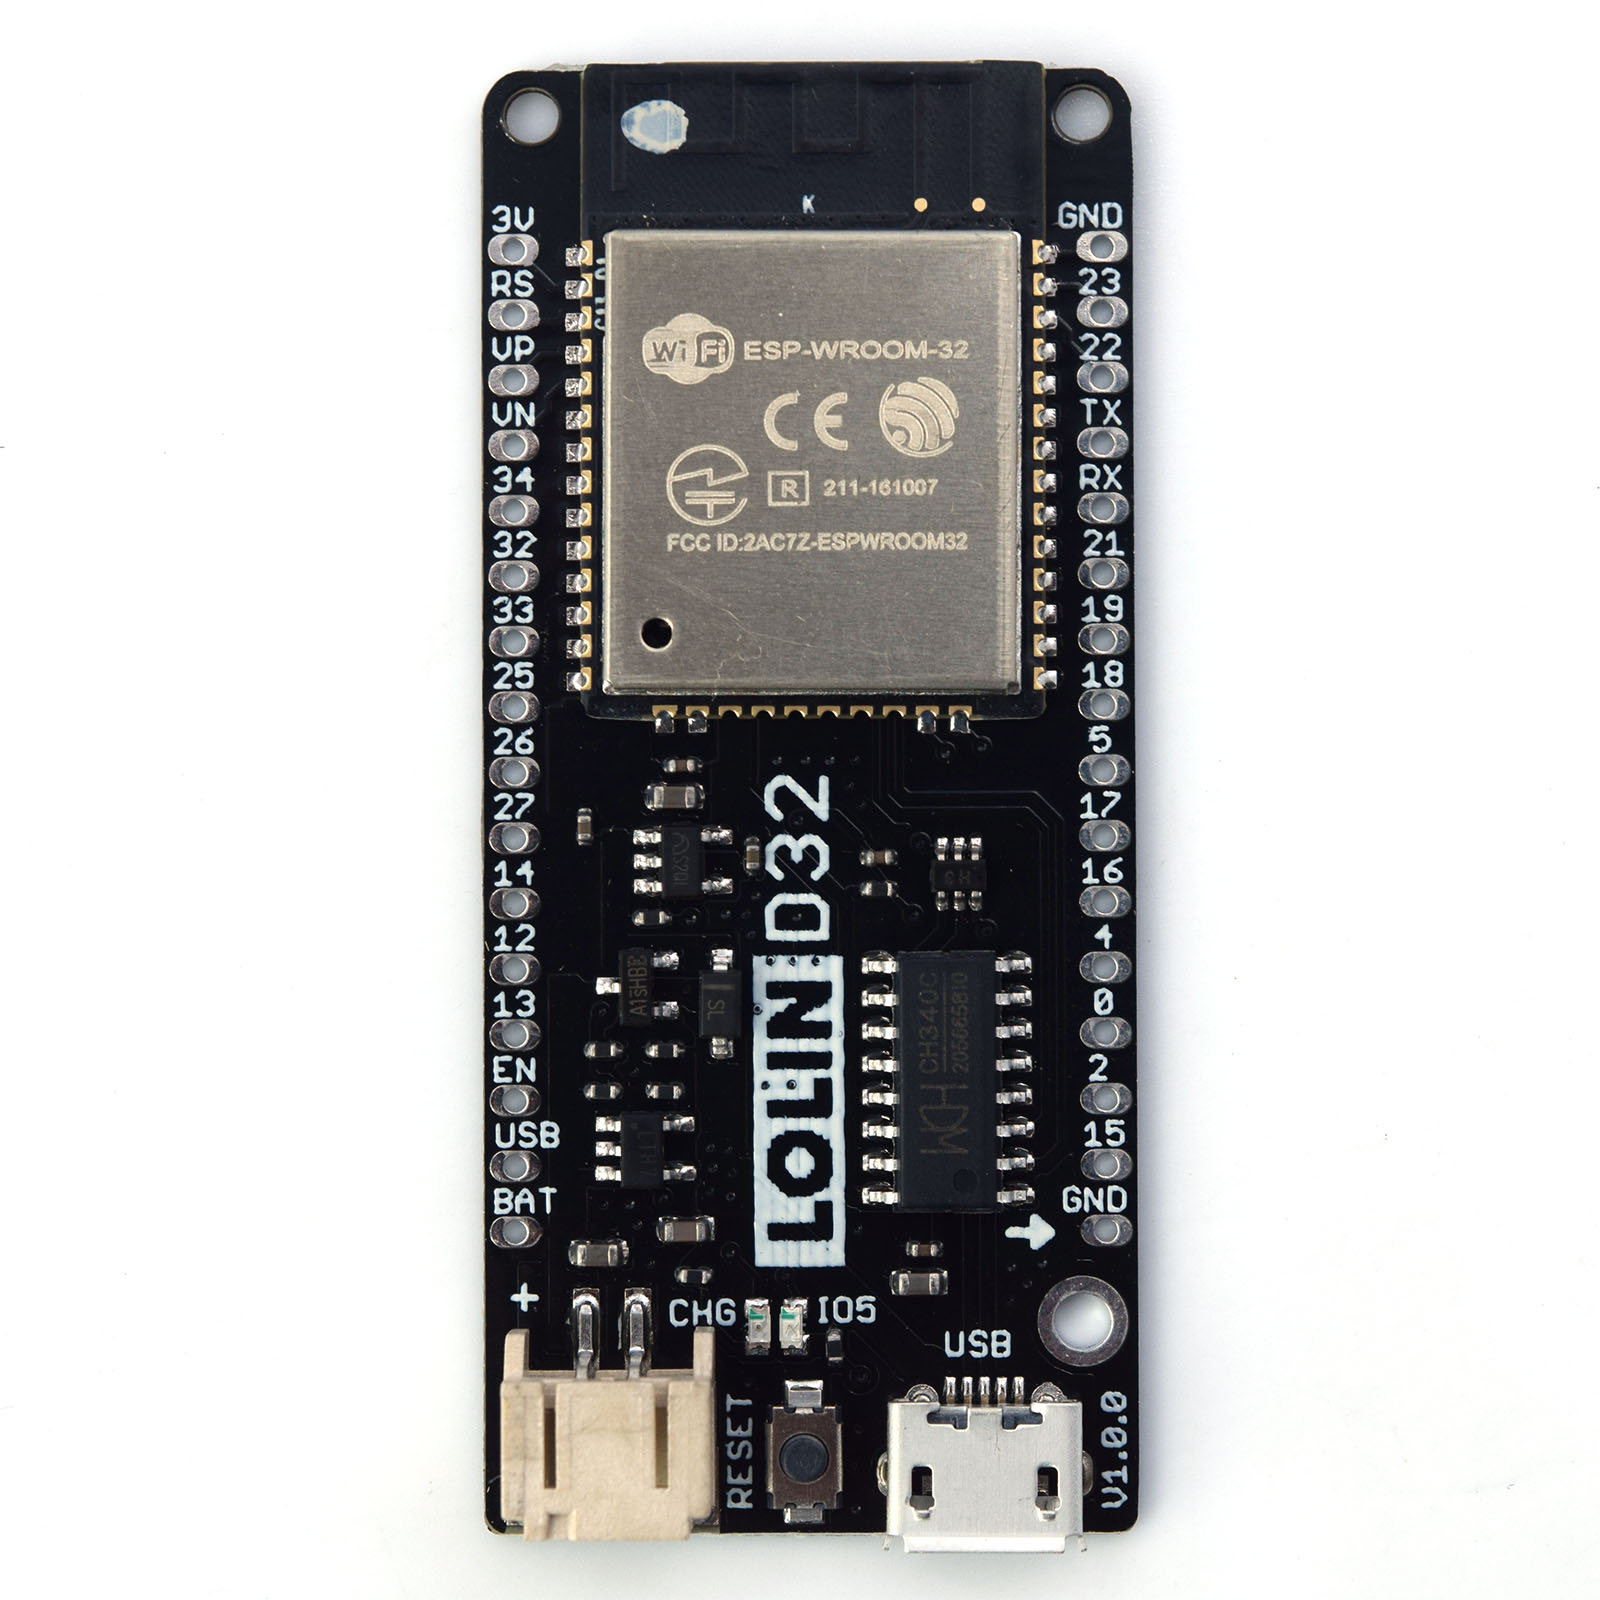
\includegraphics[scale=0.5]{images/d32_lolin}
    \caption{ESP32 pločica (Izvor:~\cite{wemos-docs})}
\end{figure}

Uz glavnu pločicu potreban je i takozvani \textit{power shield} koji omogućava napajanje od 12V\@.
Komponenta nije uključena u standardni paket WEMOS D32, a potrebna je zbog električne brave koja radi na 12V\@.

\subsection{MFRC522}

Kreditne kartice sadrže RFID čip u kojem je pohranjen jedinstveni identifikator kartice (UID).
Za autorizaciju pristupa sefu potrebno je pročitati UID s čitačem RFID kartica.

\begin{figure}[h!]
    \centering
    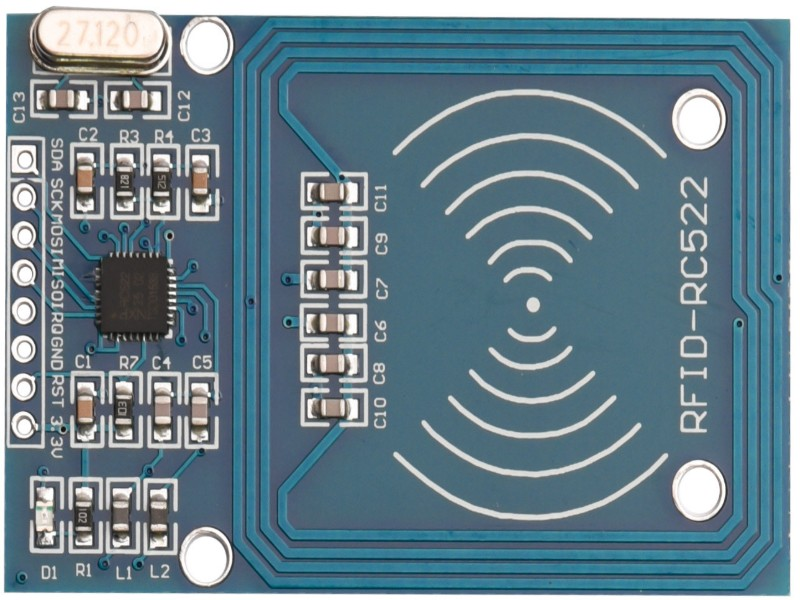
\includegraphics[scale=0.25]{images/mfrc522}
    \caption{MFRC522 čitač (Izvor:~\cite{mfrc522-eradionica})}
\end{figure}

\subsection{Mikroprekidač}

Magnetski mikroprekidač je dvodijelna komponenta koja zatvara strujni krug kad su obje komponente blizu jedna drugoj
(oko 20 milimetara).
Jednostavna komponenta koja služi za određivanje stanja sefa (otvoren ili zatvoren).
Proizvođač je tvrtka \textit{SparkFun}.

\begin{figure}[h!]
    \centering
    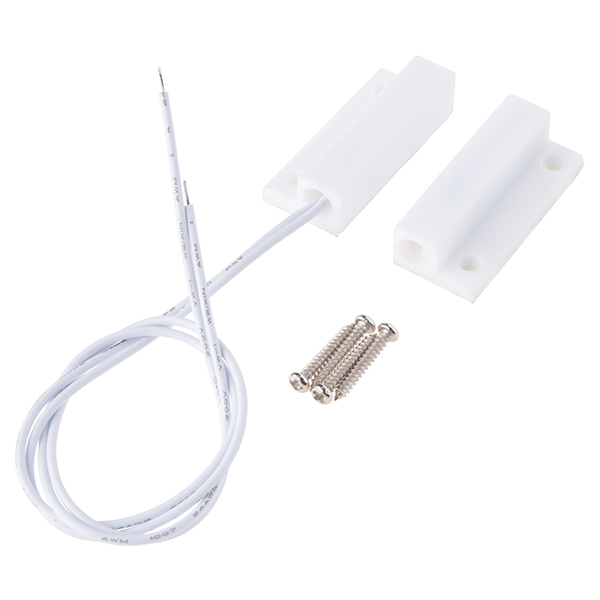
\includegraphics{images/magnetic-switch}
    \caption{Magnetski mikroprekidač (Izvor:~\cite{sparkfun-switch})}
\end{figure}

\pagebreak

\subsection{RGB LED}

LED dioda koja podržava RGB spektar boja.
Komponenta služi kao informacija korisniku o uspješnosti otvaranja sefa.

\begin{figure}[h!]
    \centering
    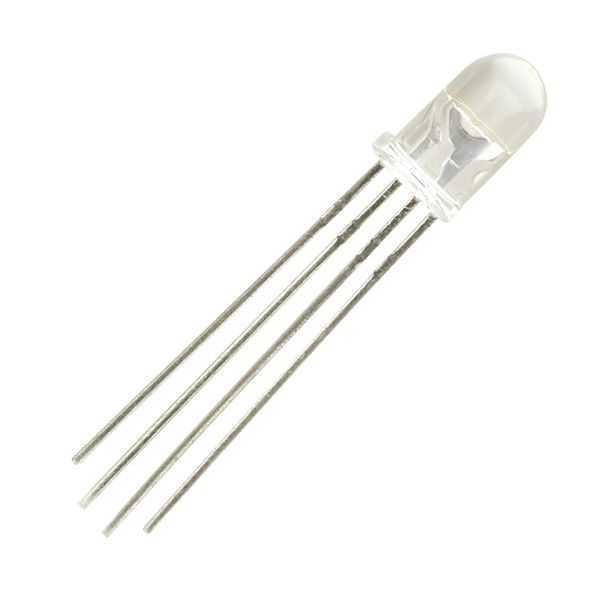
\includegraphics[scale=0.7]{images/rgb-led}
    \caption{RGB LED (Izvor:~\cite{robotistan-led})}
\end{figure}

\subsection{Brava i relej}

Električna brava koja radi na 12V i 500mA\@.
Kad relej zatvori strujni krug brava se otvara i omogućava korisniku pristup sefu.

\begin{figure}[h!]
    \centering
    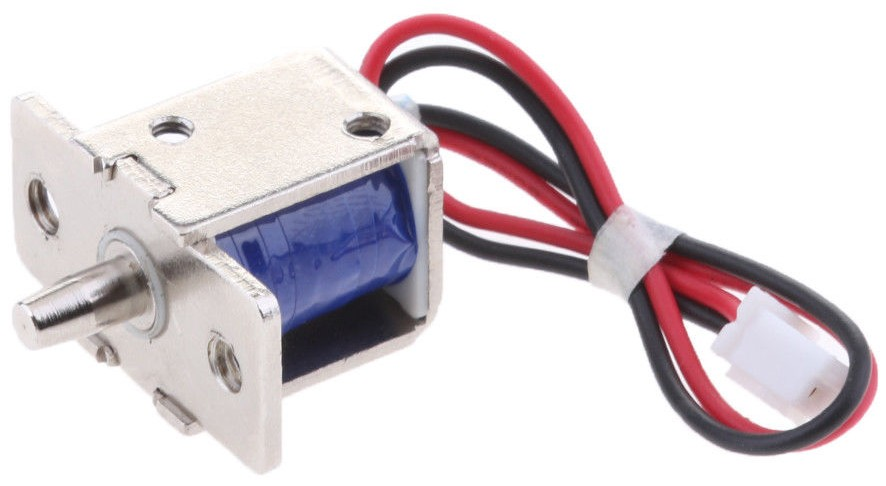
\includegraphics[width=200pt]{images/door-lock}
    \caption{Brava (Izvor:~\cite{ebay-doorlock})}
\end{figure}

\begin{figure}[h!]
    \centering
    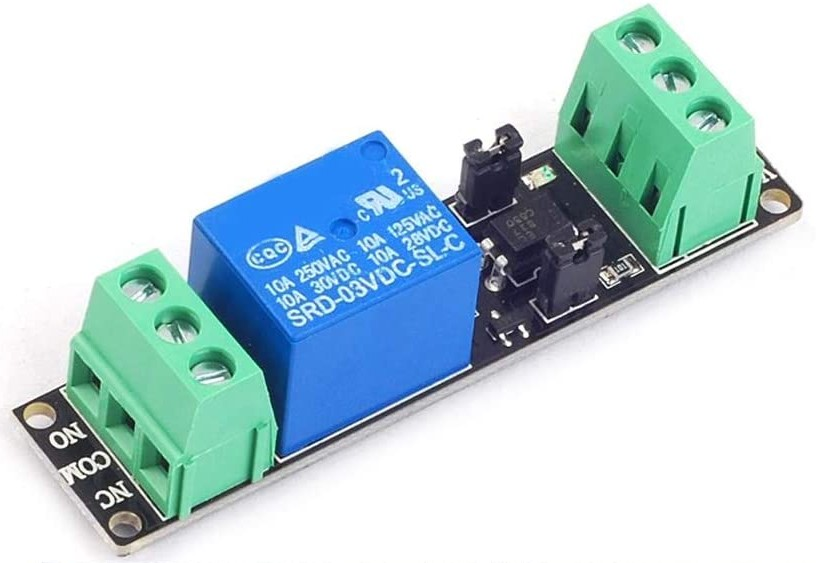
\includegraphics[width=200pt]{images/relay}
    \caption{Relej (Izvor:~\cite{amazon-relay})}
\end{figure}

\pagebreak

\subsection{Napajanje}

Većina komponenti zahtjeva 3.3V napajanje, no električna brava radi na 12V pa zahtjeva vanjsko napajanje.
Potrebno je vanjsko napajanje koje pretvara 220V u 12V\@.

\begin{figure}[h!]
    \centering
    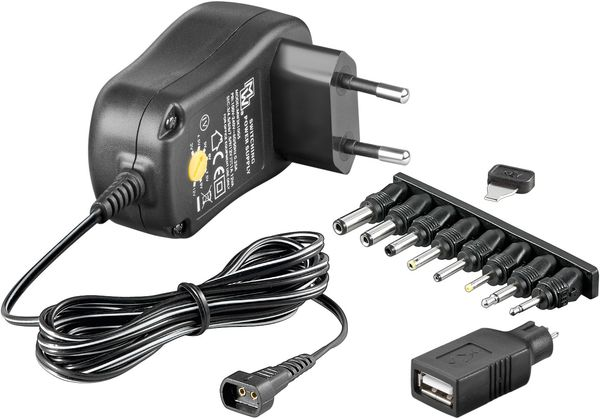
\includegraphics[scale=0.4]{images/power-supply}
    \caption{Napajanje (Izvor:~\cite{chipoteka-power-supply})}
\end{figure}

\subsection{Schema komponenti}

\begin{figure}[h!]
    \centering
    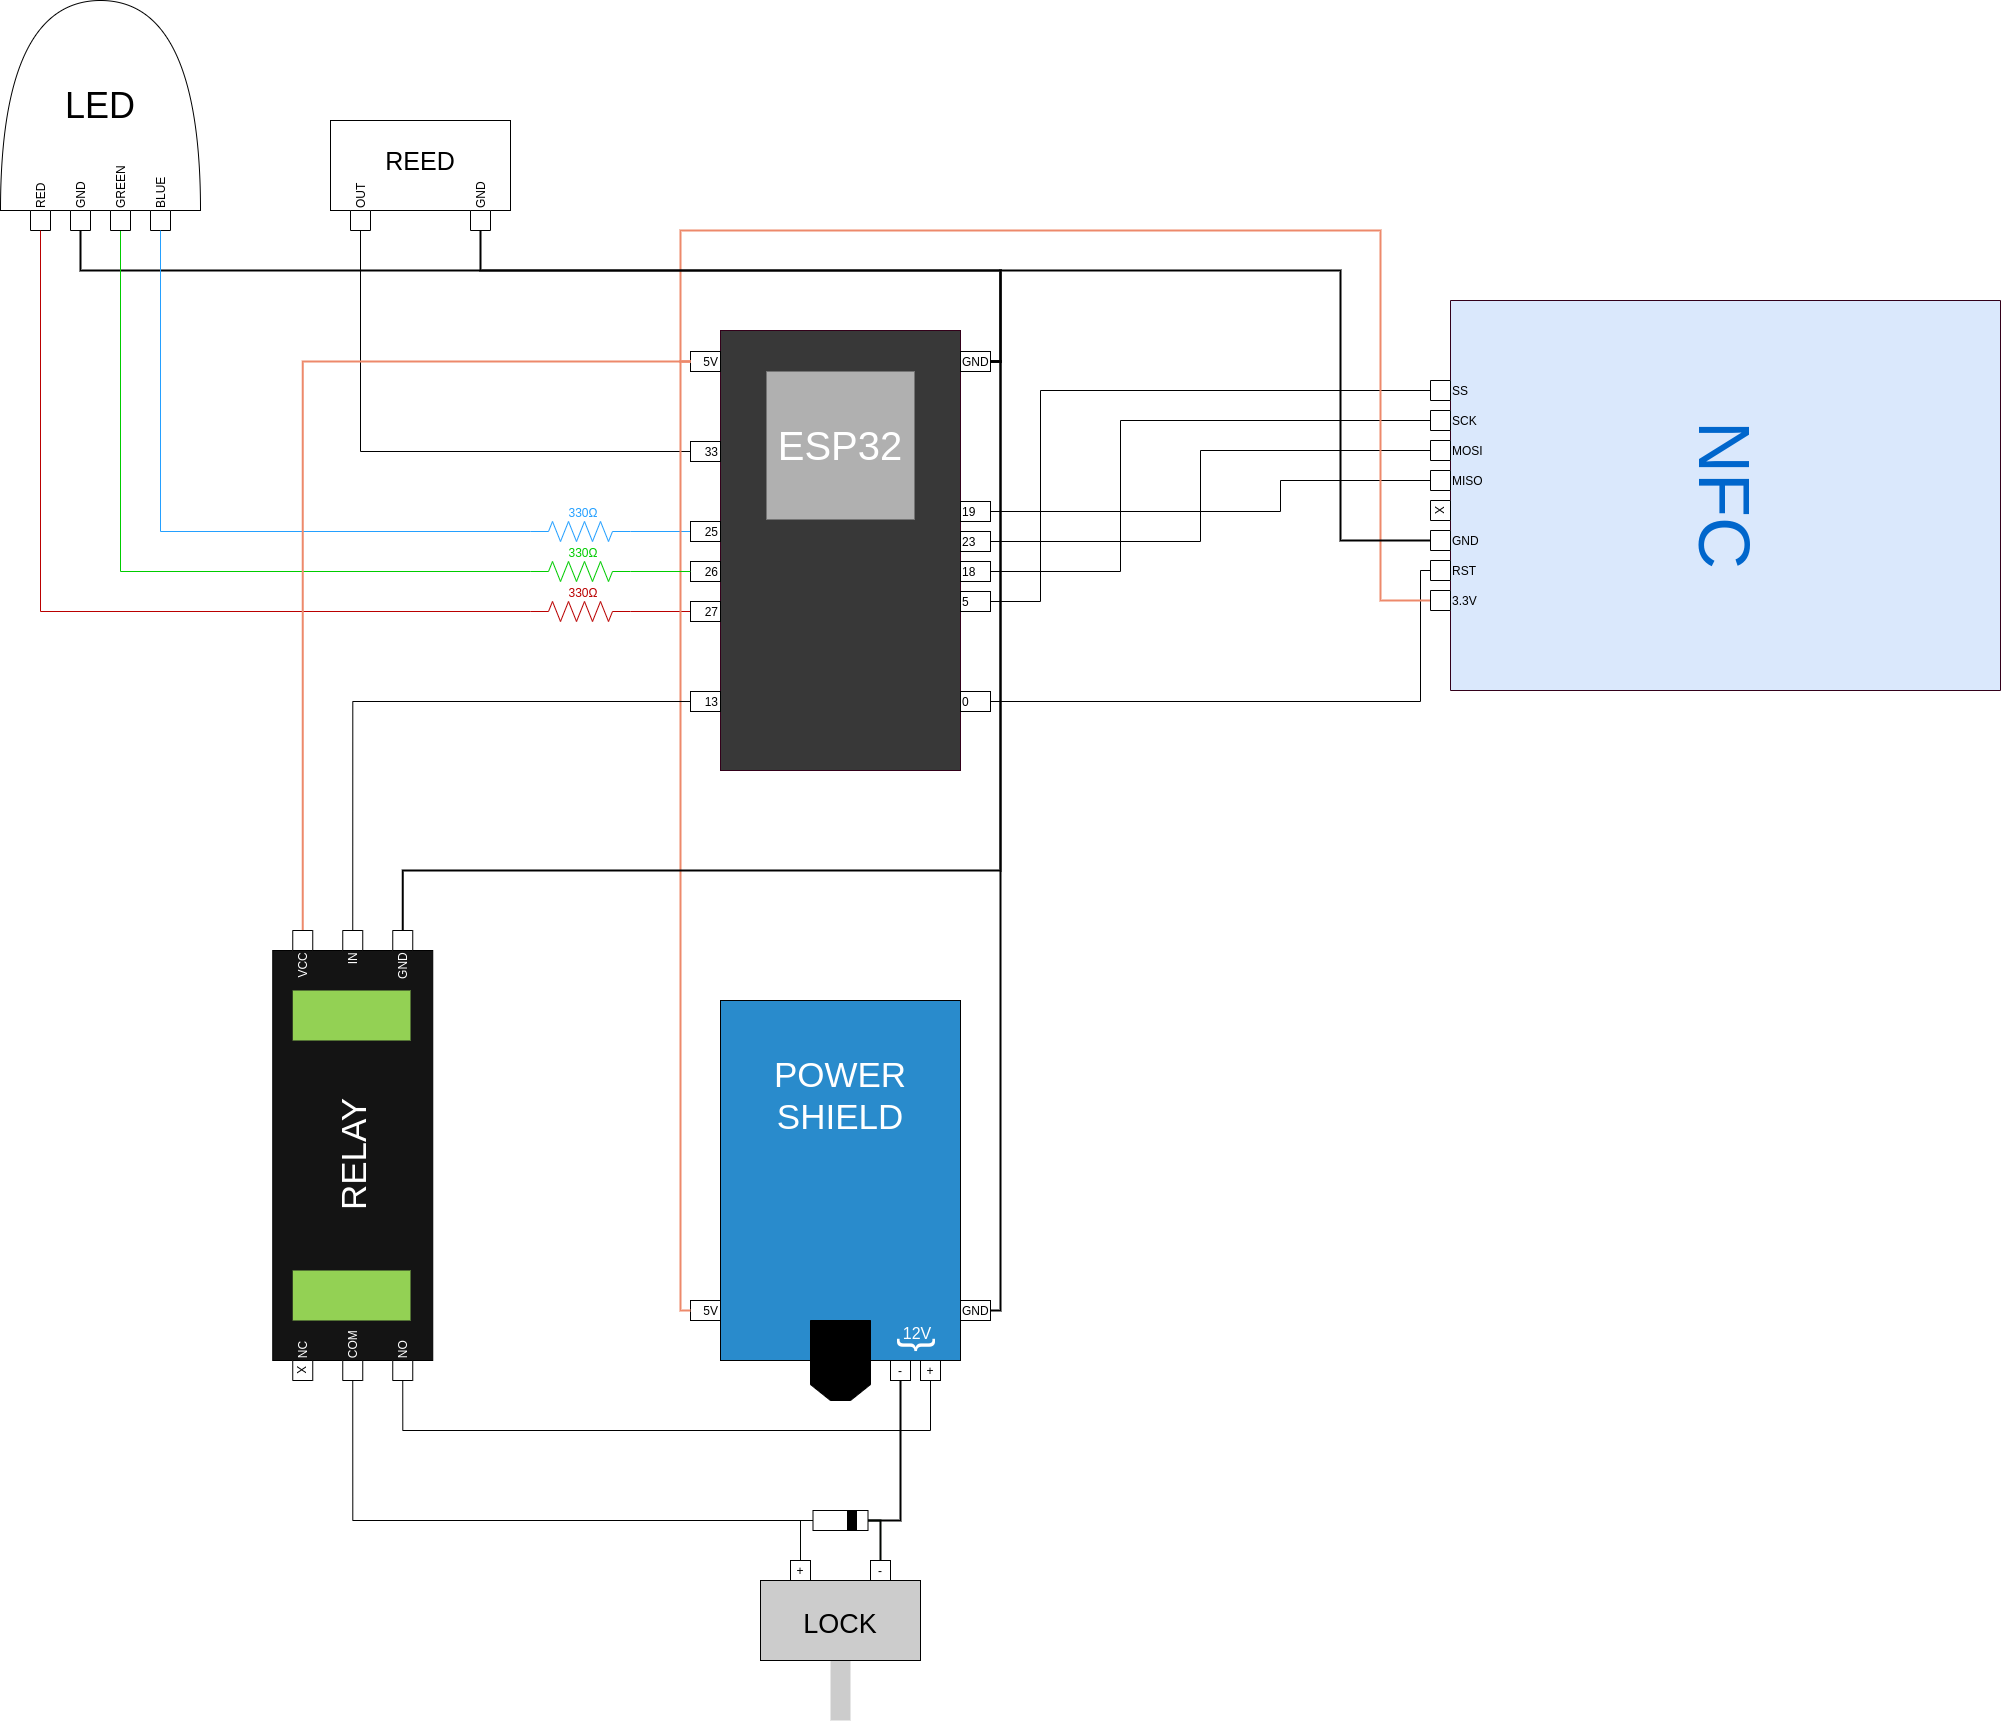
\includegraphics[width=\textwidth]{images/component-schema}
    \caption{Schema komponenti}
    \label{fig:component-schema}
\end{figure}

\pagebreak

Na slici~\ref{fig:component-schema} u centru svega nalazi se ESP32 mikrokontroler.
Pinovi s desne strane mikrokontrolera (19, 23, 18, 5 i 0) potrebni su za komunikaciju s NFC čitačem.
Sve tri boje LED diode (crvena, zelena i plava) su u upotrebi, a između svake žice i mikrokontrolera nalazi se
otpornik od 300 oma.
Magnetski mikroprekidač najjednostavnija je komponenta, a informacije o stanju pruža mikrokontroleru na pinu broj 33.
Upravljanje bravom se ne izvodi direktno već pomoću releja na pinu broj 13.
Relej i brava zahtijevaju napajanje i uzemljenje od 12V s \textit{power shield-a}.
Dovodom struje na \textit{IN} ulaz releja zatvara se strujni krug i propušta se struja na \textit{COM} izlaz koji je
povezan s pozitivnim polom brave i otključava bravu.

Testiranjem sefa utvrđeno je neočekivano ponašanje.
Uzastopno otključavanje brave dovodi do nemogućnosti čitanja kartice i podataka s iste.
Ispitivanjem je utvrđeno da mikrokontroler radi pravilno, dok NFC čitač ne prepoznaje ranije prepoznatu karticu.
Nema uzorka u pojavljivanju ovakvog ponašanja (npr.\ nakon X uspješnih čitanja ili X minuta dolazi do nepravilnog rada)
već se događa nasumično.

Brava uvlači klin pomoću elektromagnetske induktivne zavojnice.
Dovodom struje na zavojnicu električna energija se pretvara u magnetsku i tvori magnetsko polje.
Odvodom struje s polova brave magnetsko polje se ruši i stvara naponski impuls obrnutog polariteta~\cite{flyback-diode}.
Elektroni promjene smjer kretanja i, na sreću, samo privremeno poremete rad NFC čitača.
Nemoguće je spriječiti promjenu smjera kretanja, no moguće je ograničiti kretanje.
Za to je potrebna takozvana \textit{flyback} dioda koja propušta jedan smjer, a blokira obrnuti smjer kretanja
~\cite{flyback-diode}.
Na slici~\ref{fig:component-schema} kod kontakata brave nalazi se \textit{flyback} dioda.
Na taj način elektroni s obratnim smjerom kretanja ne dolaze do ostalih komponenti sefa i NFC čitač radi pravilno.

\pagebreak

\subsection{Integracija komponenti u sef}

Mikrokontroler, \textit{power shield}, relej, \textit{flyback} dioda i ožičenje zalemljeni su na plastičnu pločicu,
a pločica je pričvršćena za kutiju.
NFC čitač, brava i utor za bravu, mikroprekidač i RGB LED dioda direktno su pričvršćeni za kutiju.

\begin{figure}[h!]
    \centering
    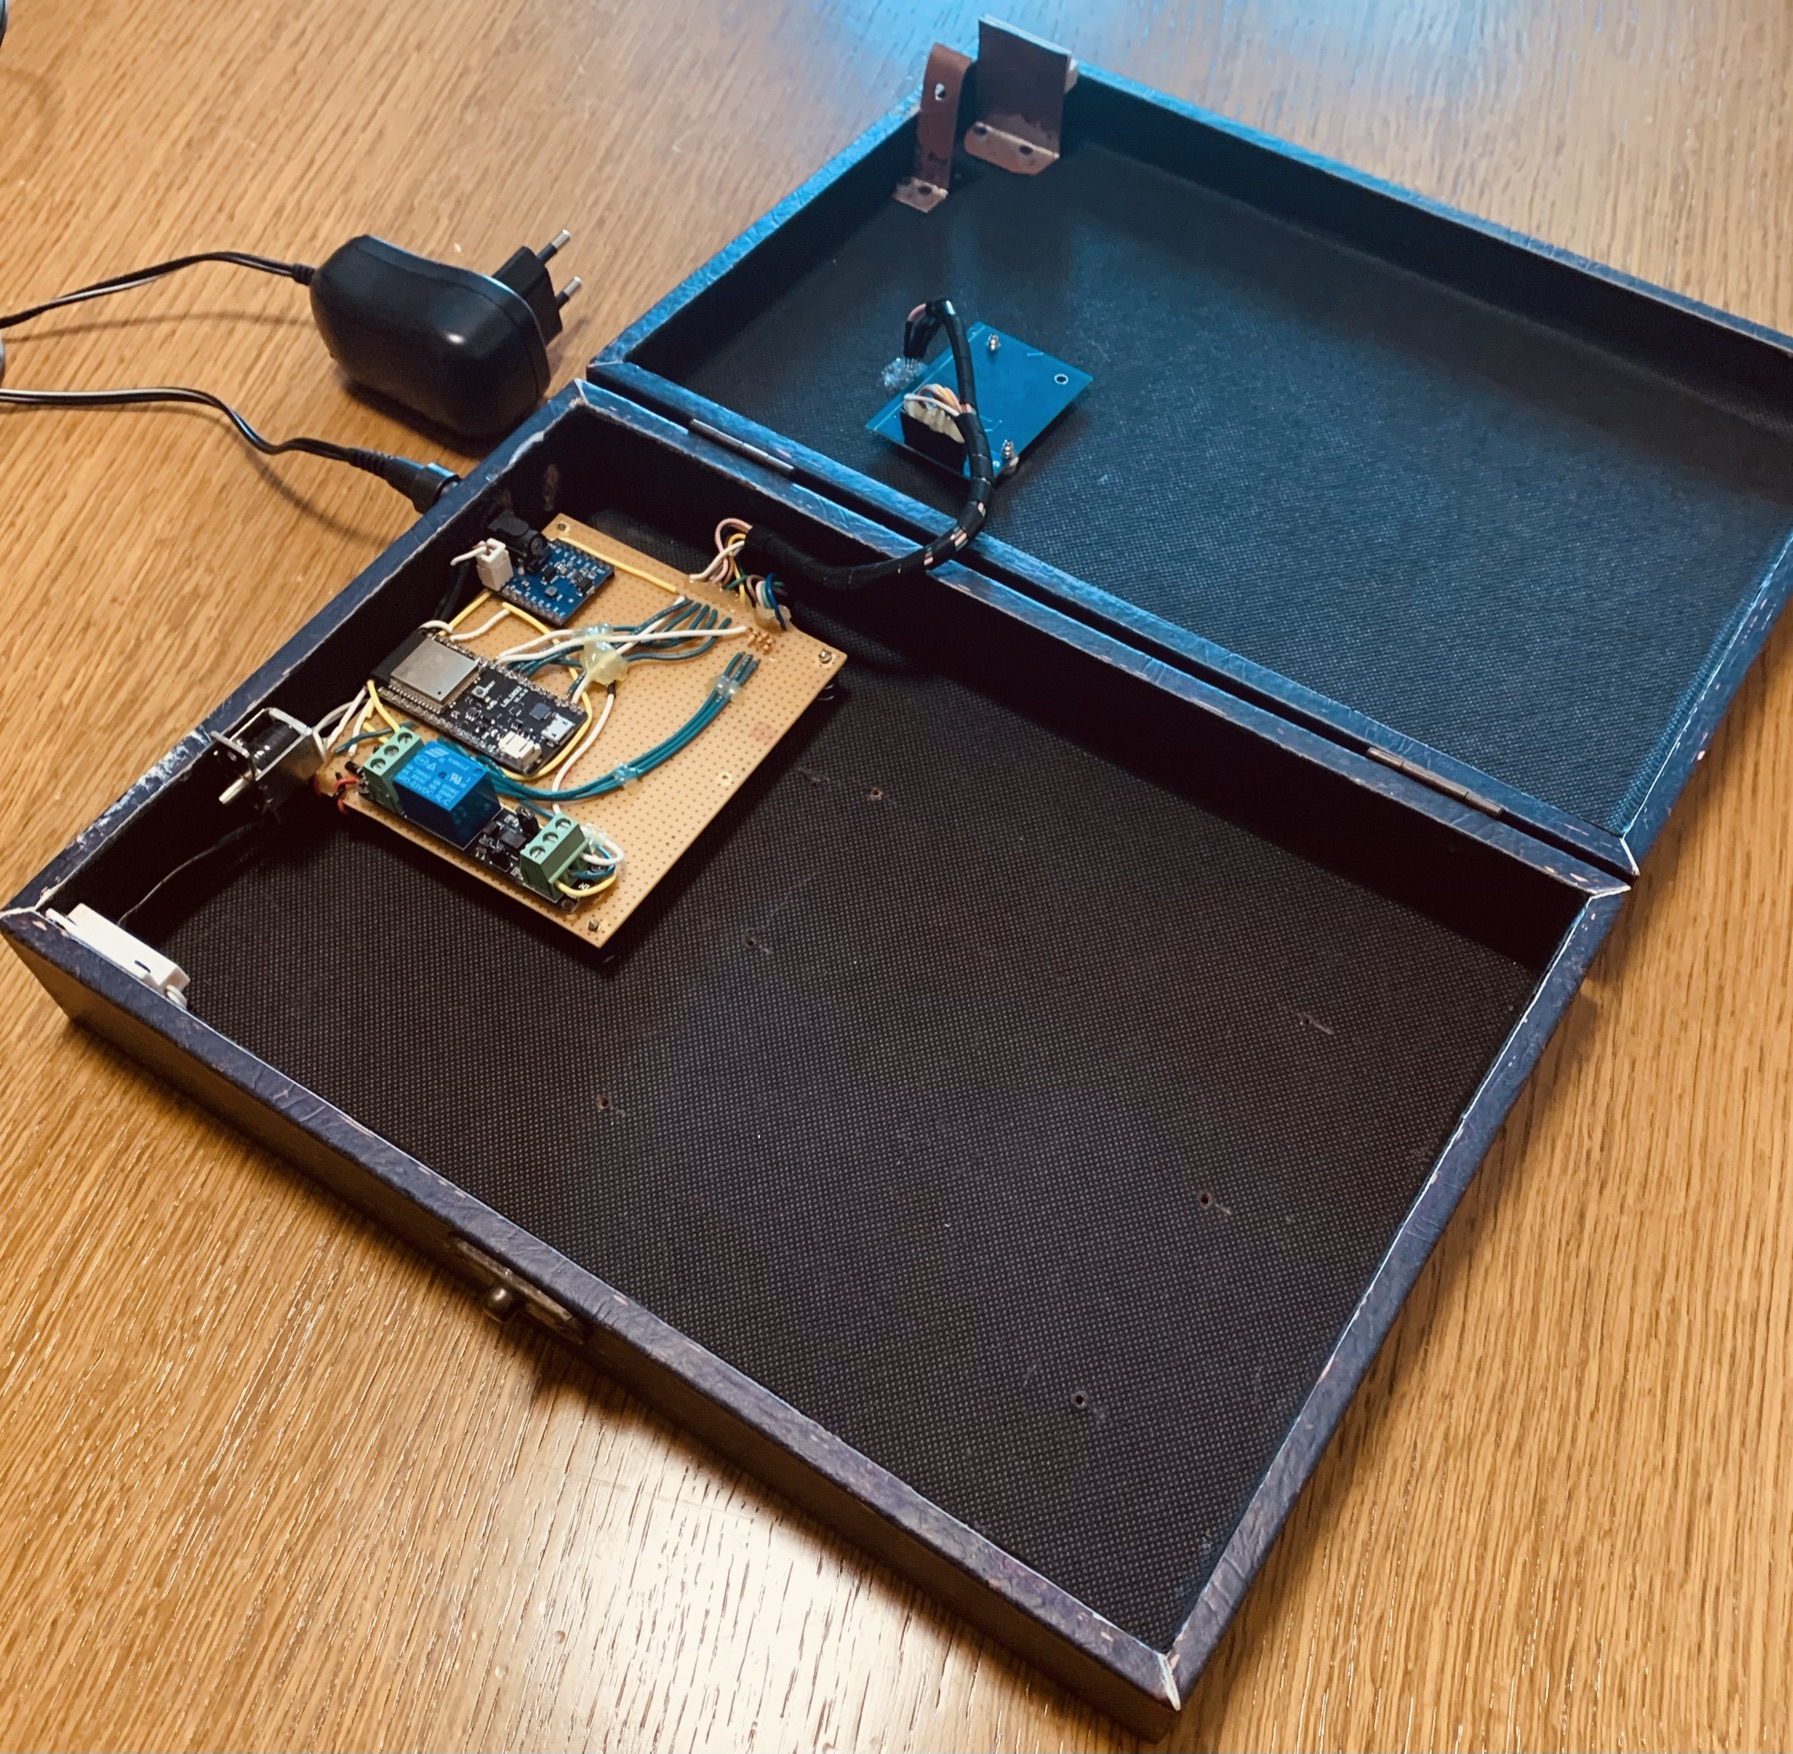
\includegraphics[width=\textwidth]{images/integrated-components}
    \caption{Schema komponenti}
\end{figure}
